%!TEX root = lec08_nosql.tex

%
%--------------------------------------------------------------------------------------------------------------
%

\begin{frame}{Distributed Transactions}

Nodes in the cluster execute two kinds of transactions:

\begin{itemize}[-,noitemsep,topsep=-10pt]
\item \textbf{\alert{Local transactions}} only read/write data on the node running the transaction.
\item \textbf{\alert{Global transactions}} read/write data on multiple nodes.
\end{itemize}

\vskip2em

\begin{columns}[onlytextwidth]
\begin{column}{0.55\textwidth}
The \textbf{transaction coordinator} synchronizes the individual (local) transactions running on different nodes via the network.
\end{column}
\begin{column}{0.45\textwidth}
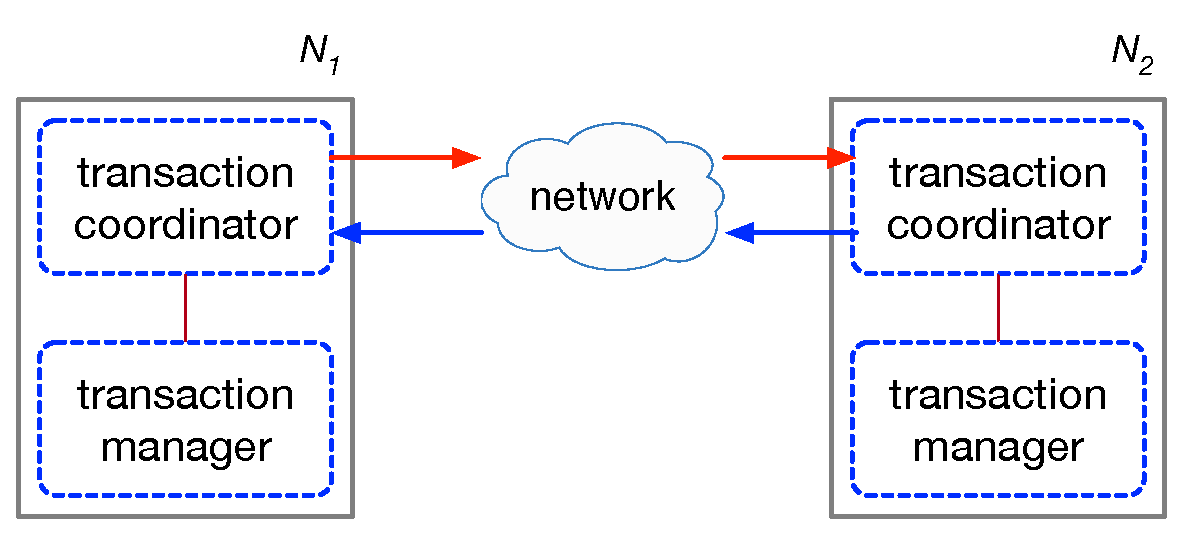
\includegraphics[width=1\textwidth]{figures/transaction_coordination.eps}
\end{column}
\end{columns}

\vskip1em

The \textbf{transaction manager} is responsible for logging and concurrency control \alert{only within the node where it runs}.

\end{frame}

%
%--------------------------------------------------------------------------------------------------------------
%

\begin{frame}{Two-Phase Commit Protocol (2PC) without failures}

2PC ensures transactions commit \textbf{if and only} all replicas are consistent. Assume node $N_1$ (with transaction coordinator $\mathit{TC}_1$) starts transaction $T_x$.

\begin{enumerate}[(1),noitemsep,topsep=-10pt]
\item $\mathit{TC}_1$ periodically sends messages to all other $\mathit{TC}_i$ that are affected by the transaction, e.g., so that they write the new values to their logs, etc.

\item \textbf{\alert{Phase 1}}: starts when the transaction is ready to commit; $\mathit{TC}_1$ writes \lstinline[style=cmput391]!<prepare Tx>! to its log, flushes its log, and sends a \textbf{prepare} message to all other $\mathit{TC}_i$ involved.\\
~~ All replicas write \lstinline[style=cmput391]!<ready Tx>! to their log and respond to $\mathit{TC}_1$ that they are ready.

\item \textbf{\alert{Phase 2}}: starts when $\mathit{TC}_1$ gets the ok from \underline{all replicas}, it writes \lstinline[style=cmput391]!<commit Tx>! to its log, flushes its log, and sends a commit message to all other $\mathit{TC}_i$.
\end{enumerate}
\end{frame}


%
%--------------------------------------------------------------------------------------------------------------
%

\begin{frame}{2PC timeline}
\begin{center}
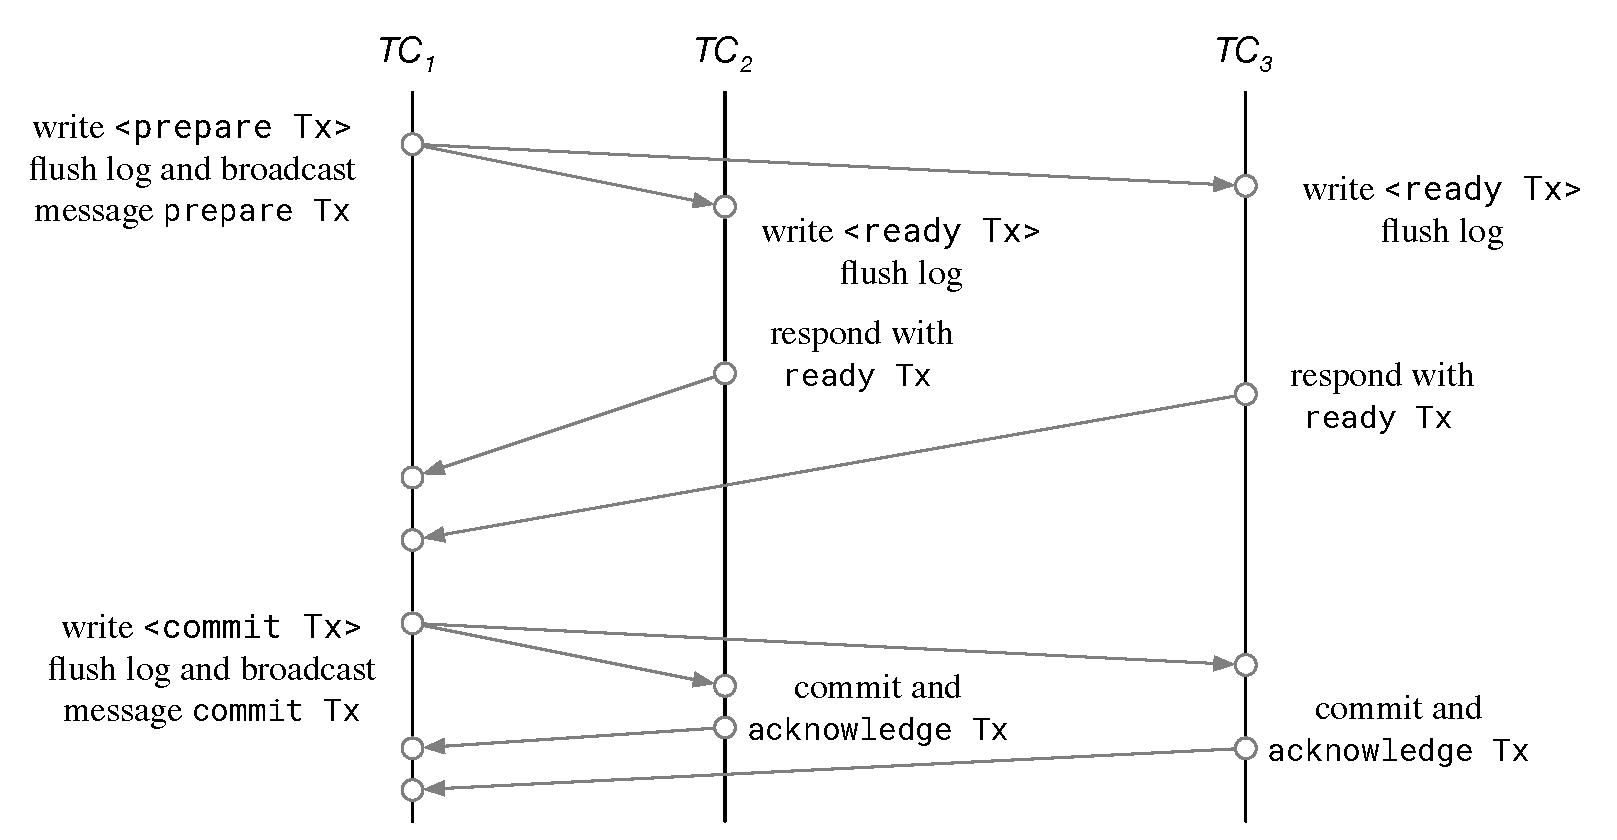
\includegraphics[width=\textwidth]{figures/2PC_example.eps}
\end{center}

$\mathit{TC}_2$ and $\mathit{TC}_3$ are the replicas of $\mathit{TC}_1$
\end{frame}

%
%--------------------------------------------------------------------------------------------------------------
%

\begin{frame}{2PC: correctness}
Rule \#1: $\mathit{TC}_1$ will only start the attempt to commit if all replicas respond with a \lstinline[style=cmput391]!<ready Tx>! message.

 If a replica cannot commit or does not respond after some time limit, the transaction is aborted and all replicas are notified to abort.

\vskip1.5em

Rule \#2: $\mathit{TC}_1$ knows all replicas are synchronized once they all respond with a \lstinline[style=cmput391]!<acknowledge Tx>! message.

\vskip1.5em

The protocol deals with different kinds of failures both in the coordinator node or in the replica node.
\end{frame}


%
%--------------------------------------------------------------------------------------------------------------
%

\begin{frame}{2PC: replica failure}

If the coordinator $\mathit{TC}_1$ detects that replica node $N_j$ failed \textbf{before} responding with \lstinline[style=cmput391]!<ready Tx>!, it assumes the replica is not ready and aborts the transaction everywhere, and no inconsistencies arise.

\vskip2em

If the coordinator $\mathit{TC}_1$ detects that replica node $N_j$ failed \textbf{after} responding with \lstinline[style=cmput391]!<ready Tx>!, it continues with the protocol with the other replicas, ignoring the node failure.

Once the failed replica $N_j$ is back up, it performs a crash recovery algorithm (next slide).
\end{frame}

%
%--------------------------------------------------------------------------------------------------------------
%

\begin{frame}{2PC: crash recovery --- replica}

Upon restart, replica $N_j$ checks its log to undo/redo transactions almost as in the single-node case (recall undo/redo logging from before). For each transaction $T_x$ in the log:

\begin{itemize}[-,noitemsep,topsep=-5pt]
\item If \lstinline[style=cmput391]!<commit Tx>! is found in the log, \textbf{redo} $T_x$.
\item If \lstinline[style=cmput391]!<abort Tx>! is found in the log, \textbf{undo} $T_x$.
\item If only \lstinline[style=cmput391]!<ready Tx>! is found in the log, then the replica must \alert{consult the transaction coordinator} $\mathit{TC}_1$ to figure out the if the transaction committed or aborted.
\begin{itemize}[-,topsep=-10pt]
\item If the coordinator is unreachable, $N_j$ queries all other replicas to check the status of the transaction.
\item Until then, $N_j$ \textbf{neither} commits nor aborts.
\end{itemize}
\item If not even \lstinline[style=cmput391]!<ready Tx>! is in the log, the replica did not respond (and the transaction has been aborted by the coordinator), so the replica aborts the transaction.
\end{itemize}
\end{frame}

%
%--------------------------------------------------------------------------------------------------------------
%

\begin{frame}{2PC: coordinator failure}

If the coordinator fails or becomes unavailable during the execution of the transaction, the replicas continue executing the transaction to the extent possible:
\begin{itemize}[-,noitemsep,topsep=-5pt]
\item If at least one replica wrote \lstinline[style=cmput391]!<commit Tx>! to its log, then all active replicas proceed to commit the transaction.
\item If an active replica wrote \lstinline[style=cmput391]!<abort Tx>!, then all active replicas must abort.
\item If at least one replica \alert{does not} have \lstinline[style=cmput391]!<ready Tx>! in its log, the coordinator cannot have started the commit phase. In this case, the replicas assume the coordinator decided to abort (based on timeout) and they all abort.
\item If all replicas have only the \lstinline[style=cmput391]!<ready Tx>! in their log, then the replicas must \alert{wait for the transaction coordinator} $\mathit{TC}_1$ to figure out the if the transaction committed or aborted.
\end{itemize}
\end{frame}

%
%--------------------------------------------------------------------------------------------------------------
%

\begin{frame}{2PC: crash recovery --- coordinator}

The crash recovery for the coordinator is identical to that of a replica $N_j$:

\begin{itemize}[-,noitemsep,topsep=-5pt]
\item Redo and commit transactions marked \lstinline[style=cmput391]!<commit Tx>! the log.
\item Undo and abort transactions marked \lstinline[style=cmput391]!<abort Tx>! in the log.
\item Consult the replicas about transactions marked \lstinline[style=cmput391]!<ready Tx>! in the log.
\item If not even \lstinline[style=cmput391]!<ready Tx>! is in the log, the replicas did not respond before the crash, and everyone decided to abort the transaction.
\end{itemize}
\end{frame}


%
%--------------------------------------------------------------------------------------------------------------
%

\begin{frame}{Network partition and delayed transactions}

\vskip2em

\begin{columns}[onlytextwidth]
\begin{column}{0.55\textwidth}

A severe network failure might partition the system into two disconnected subsystems.

\vskip1em

The 2PC protocol dictates how the coordinator and the replicas behave if the failure happens during the execution of a transaction.
\end{column}
\qquad\begin{column}{0.45\textwidth}
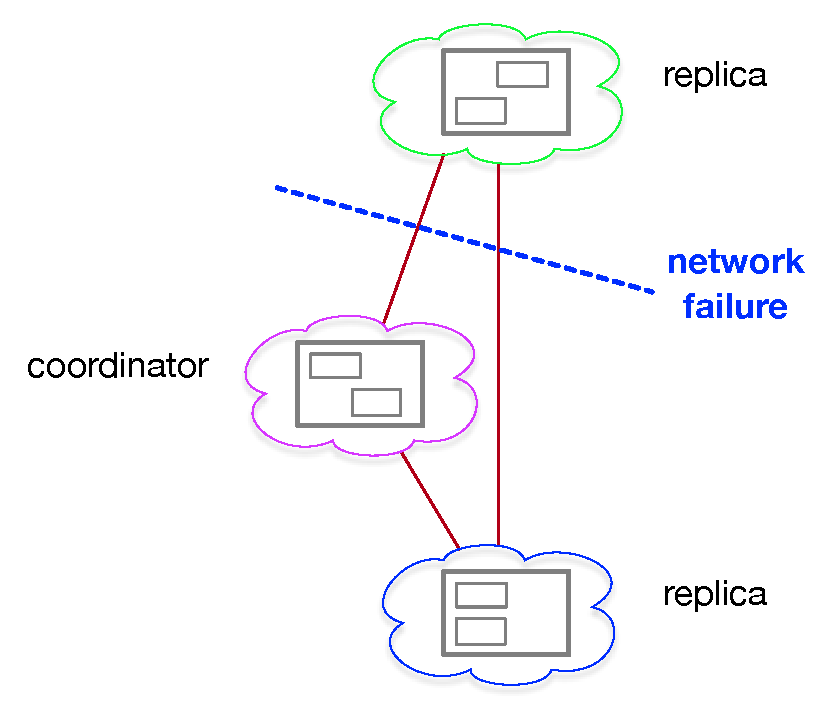
\includegraphics[width=1\textwidth]{figures/network_failure_partition.eps}
\end{column}
\end{columns}

\vskip1em

However, can the same query have a different answer depending on the node it is issued?

Also, should new transactions be accepted while the network is partitioned?

\end{frame}


%
%--------------------------------------------------------------------------------------------------------------
%

\begin{frame}

\vskip2em

\begin{columns}[onlytextwidth]
\begin{column}{0.55\textwidth}

Example: if the isolated replica could not decide whether or not to commit or abort a transaction $T_x$, it \textbf{cannot} accept new transactions that use data written by $T_x$!

\vskip1em

But what about the other nodes in the ``other half'' of the system?
\end{column}
\qquad\begin{column}{0.45\textwidth}
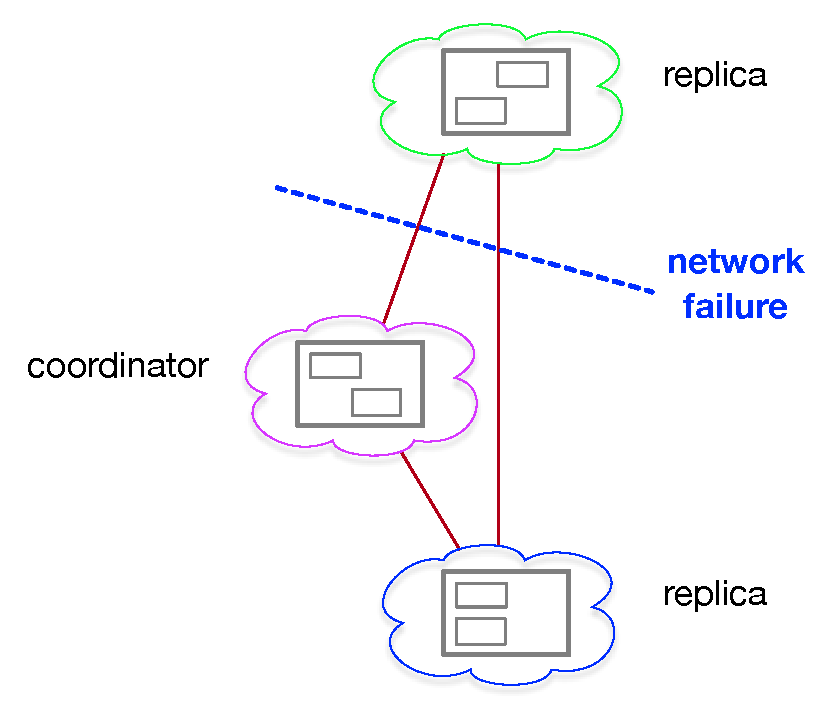
\includegraphics[width=1\textwidth]{figures/network_failure_partition.eps}
\end{column}
\end{columns}

\vskip1em

What if the network failure may last for a long time? 
\begin{itemize}[-,noitemsep]
\item Should the system stop accepting transactions? 
\item What about queries?
\end{itemize}
\end{frame}

%
%--------------------------------------------------------------------------------------------------------------
%

\begin{frame}{Accepting Transactions in a Partitioned System}


\begin{columns}[onlytextwidth]
\begin{column}{0.55\textwidth}

\begin{block}{The \alert{blocking} problem}
A node isolated from the rest of the network it may not know if a transaction committed or aborted, preventing it from accepting new transactions (e.g., to avoid uncommitted reads).
\end{block}

\end{column}
\qquad\begin{column}{0.45\textwidth}
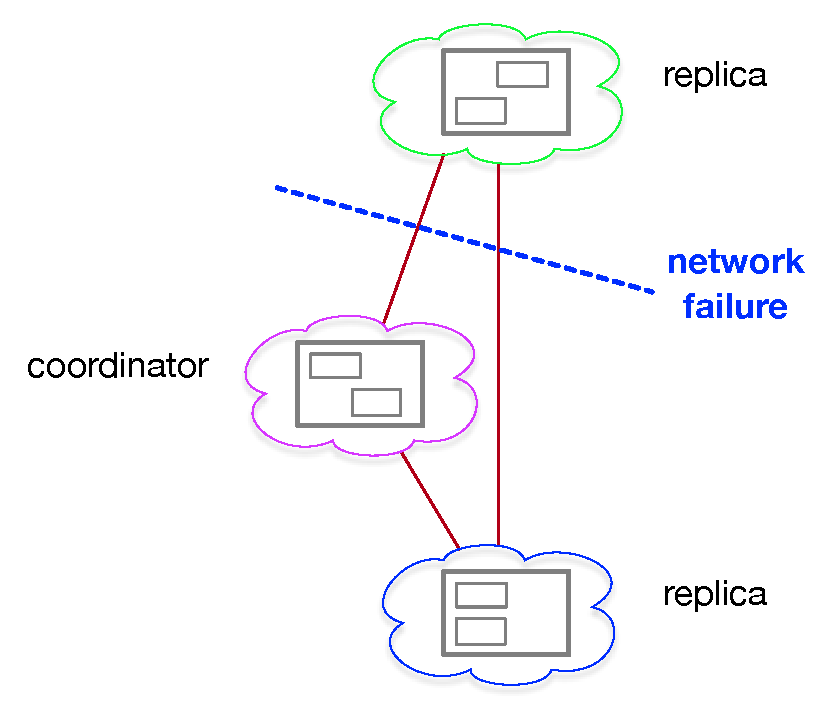
\includegraphics[width=1\textwidth]{figures/network_failure_partition.eps}
\end{column}
\end{columns}

\vskip0.75em

But distributing the data was meant to bring \textbf{\alert{high availability}}. Instead, the whole system becomes unavailable when there is a failure somewhere else.

\alert{High Availability} and \textcolor{blue}{Data Consistency} are conflicting goals...
\end{frame}


%
%--------------------------------------------------------------------------------------------------------------
%

\begin{frame}{Eventual Consistency With Majority Locking}

\vskip2em

\begin{columns}[onlytextwidth]
\begin{column}{0.65\textwidth}
One way to allow the system to tolerate node or network failures is to allow a transaction $T_1$ to write a database element \alert{A} if it can acquire locks on the (simple) majority of the nodes with copies of \alert{A}.

\vskip1em

\textbf{Timestamps} (agreed upon at locking time) are used to record the version of \alert{A} that is written.

\vskip1em

After the update commits the system becomes inconsistent: different nodes have different ``most recent'' values of the same element.
\end{column}
\begin{column}{0.3\textwidth}
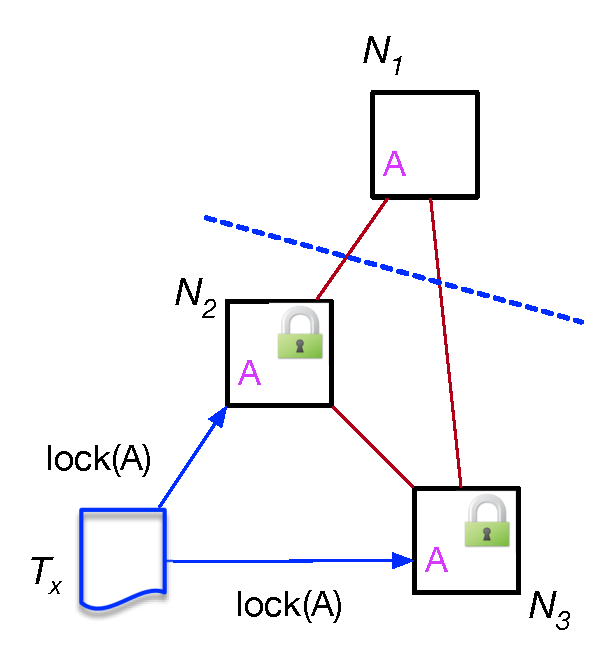
\includegraphics[width=\textwidth]{figures/majority_locking_A.eps}

\vskip1em

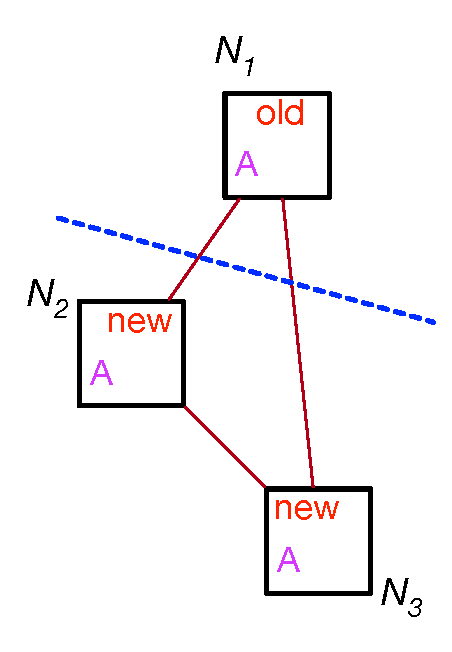
\includegraphics[width=0.75\textwidth]{figures/majority_inconsistent_A.eps}
\end{column}
\end{columns}
\end{frame}

%
%--------------------------------------------------------------------------------------------------------------
%

\begin{frame}

\begin{columns}[onlytextwidth]
\begin{column}{0.55\textwidth}
Inconsistent data can be detected in many ways:
\begin{itemize}[-,noitemsep,topsep=-5pt]
 \item A node with a copy of \alert{A} re-joins the network after a failure and asks its peers for missed transactions.
 \item Another node requests \alert{A} from all copies and gets inconsistent answers.
\end{itemize}
\end{column}
\begin{column}{0.4\textwidth}
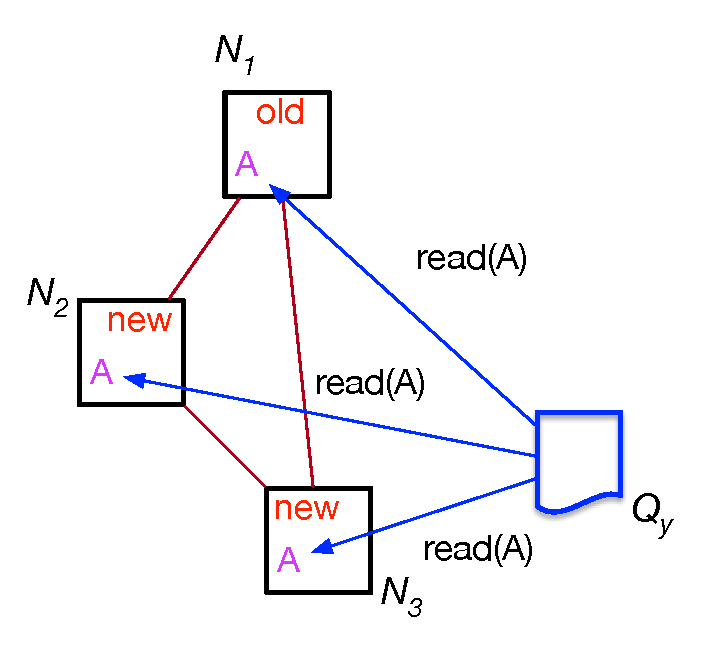
\includegraphics[width=1.1\textwidth]{figures/majority_read_all.eps}
\end{column}
\end{columns}

In summary, majority voting ensures the system remains available during the failure of a node, but incurs too many reads to work well.

\end{frame}

%
%--------------------------------------------------------------------------------------------------------------
%

\begin{frame}{The CAP ``Theorem''}

Although this is not a formal statement, it is generally accepted that no distributed database system that enforces \alert{ACID} transactions can achieve these three properties \textbf{simultaneously}:
\begin{itemize}[-,noitemsep,topsep=-10pt]
\item \alert{\textbf{C}}onsistency: all replicas have the same value.
\item \alert{\textbf{A}}vailability: the system accepts transactions at any time.
\item \alert{\textbf{P}}artition tolerance: the system operates normally even under a network partition failure.
\end{itemize}

\vskip1.5em

Instead of ACID, NoSQL systems are \textcolor{blue}{BASE}:
\begin{itemize}[-,noitemsep,topsep=-10pt]
\item \textcolor{blue}{\textbf{BA}}sically available: it works as long as the majority of the replicas are up.
\item \textcolor{blue}{\textbf{S}}oft state: inconsistencies are time-stamped.
\item \textcolor{blue}{\textbf{E}}ventually consistent: replicas do synchronize after a while.
\end{itemize}
\end{frame}

%
%--------------------------------------------------------------------------------------------------------------
%

\begin{frame}{Synchronization across data centers}

\vskip2em

\begin{columns}[onlytextwidth]
\begin{column}{0.6\textwidth}
Many applications require the data to be \alert{\textbf{distributed}} across geographically dispersed data centers to reduce the chance of critical data loss due to catastrophic failures in one location (e.g., fire in one data center).

\vskip0.75em

The 2PC protocol works on these systems as well, although network latency and connectivity can introduce significant delays in replica synchronization.

\end{column}
\qquad\begin{column}{0.4\textwidth}
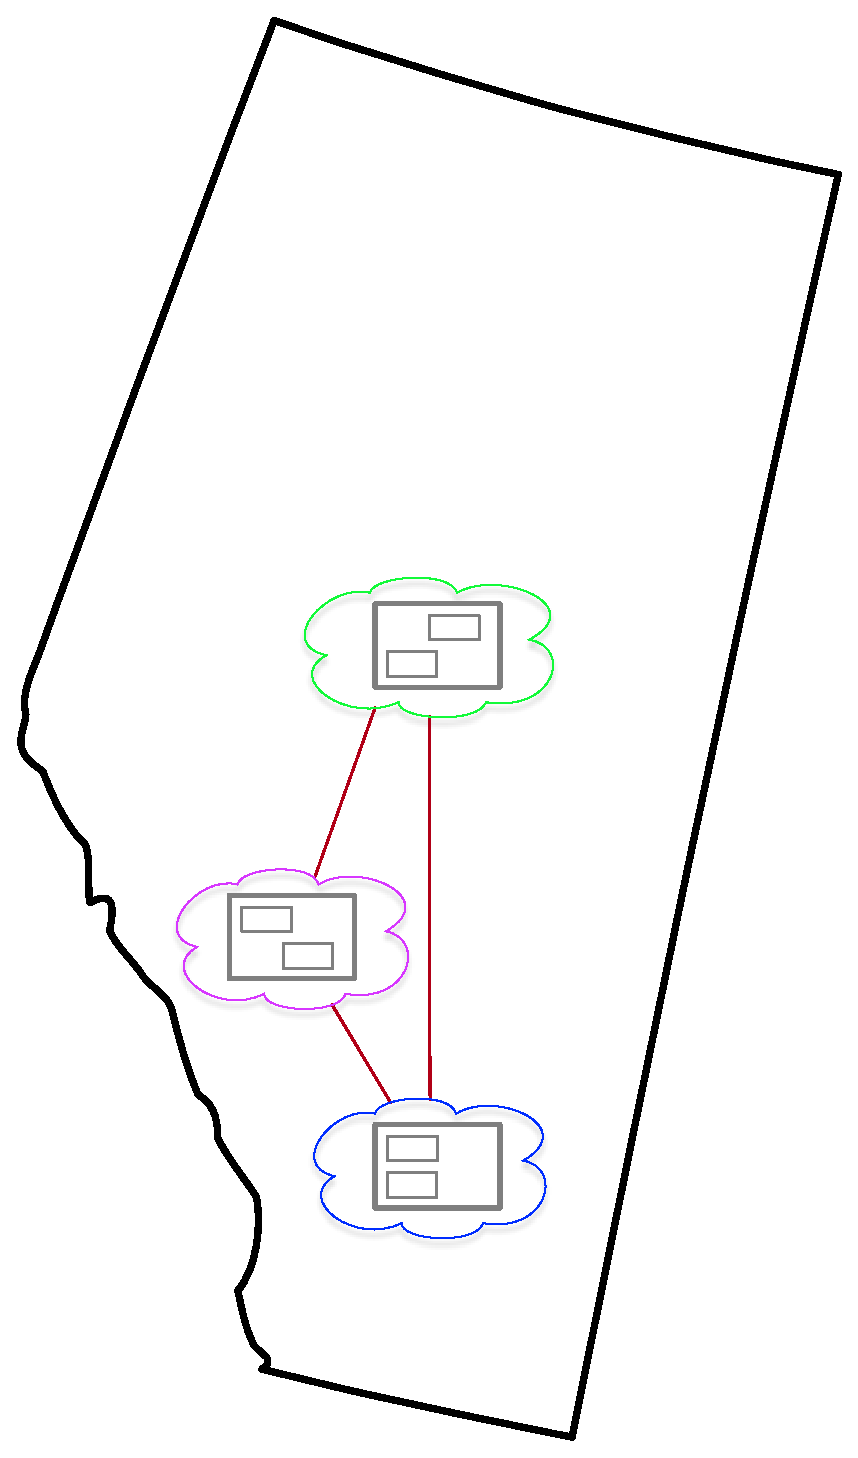
\includegraphics[width=0.75\textwidth]{figures/AB_distributed_table.eps}
\end{column}
\end{columns}

\vskip0.75em

It is up to the database administrator to evaluate the trade-offs between responsiveness and data consistency.
\end{frame}


%
%--------------------------------------------------------------------------------------------------------------
%

\begin{frame}{Moral of the story?}

If an application cannot tolerate inconsistent data (e.g., a banking application), then it will use the 2PC protocol and require all locks to be available before writing.

Most distributed applications (e.g., social networks) can tolerate inconsistent data. The worst that can happen is that users connected to different nodes (e.g., opposite coasts of Canada) of the system don't see each others posts for some time.

\end{frame}








